\let\negmedspace\undefined
\let\negthickspace\undefined
\documentclass[journal]{IEEEtran}
\usepackage[a5paper, margin=10mm, onecolumn]{geometry}
\usepackage{lmodern} % Ensure lmodern is loaded for pdflatex
\usepackage{tfrupee} % Include tfrupee package

\setlength{\headheight}{1cm} % Set the height of the header box
\setlength{\headsep}{0mm}     % Set the distance between the header box and the top of the text

\usepackage{gvv-book}
\usepackage{gvv}
\usepackage{cite}
\usepackage{amsmath,amssymb,amsfonts,amsthm}
\usepackage{algorithmic}
\usepackage{graphicx}
\usepackage{textcomp}
\usepackage{xcolor}
\usepackage{txfonts}
\usepackage{listings}
\usepackage{enumitem}
\usepackage{mathtools}
\usepackage{gensymb}
\usepackage{comment}
\usepackage[breaklinks=true]{hyperref}
\usepackage{tkz-euclide} 
\usepackage{listings}
\usepackage{gvv}                                        
\def\inputGnumericTable{}                                 
\usepackage[latin1]{inputenc}                                
\usepackage{color}                                            
\usepackage{array}                                            
\usepackage{longtable}                                       
\usepackage{calc}                                             
\usepackage{multirow}                                         
\usepackage{hhline}                                           
\usepackage{ifthen}                                           
\usepackage{lscape}
\begin{document}

\bibliographystyle{IEEEtran}
\vspace{3cm}

\title{9.9.2.28}
\author{EE24BTECH11024 - Abhimanyu Koushik}
% \maketitle
% \newpage
% \bigskip
{\let\newpage\relax\maketitle}
\textbf{Question:}\\
Find the area of region bounded by the line $x=2$ and the parabola $y^2=8x$\\
\textbf{Solution:}
\begin{table}[h!]    
  \centering
  \begin{tabular}[12pt]{ |c|c|c|}
    \hline
    \textbf{Symbol} & \textbf{Value} & \textbf{Description} \\
    \hline
    $\vec{A}$ & \myvec{6\\5} & First point\\
    \hline 
    $\vec{B}$ & \myvec{-4\\3} & Second point\\
    \hline
    $\vec{Y}$ & \myvec{0\\$y$} & Point on Y-Axis equidistant from A and B\\
    \hline
    \end{tabular}

  \caption{Variables Used}
  \label{tab1-1.9-6}
\end{table}\\
The equation of a parabola in Matrix form is
\begin{align}
\vec{x}^\top\vec{V}\vec{x} + 2\vec{u}^\top\vec{x} + f = 0
\end{align}
The equation of a line in vector form is
\begin{align}
\vec{x}&=\vec{h}+\kappa\vec{m}
\end{align}
For the given parabola $y^2=8x$, The values of $\vec{V}$,$\vec{u}$,$f$ are
\begin{align}
\vec{V}&=\myvec{0 & 0\\0 & 1}\\
\vec{u}&=\myvec{-4\\0}\\
f&=0
\end{align}
For the given line $x=2$, The values of $\vec{h}$, $\vec{m}$ are
\begin{align}
\vec{h}&=\myvec{2\\0}\\
\vec{m}&=\myvec{0\\1}
\end{align}
Substituing the line equation in parabola equation gies the values of $\kappa$
\begin{align}
\brak{\vec{h}+\kappa\vec{m}}^\top\vec{V}\brak{\vec{h}+\kappa\vec{m}} + 2\vec{u}^\top\brak{\vec{h}+\kappa\vec{m}} + f &= 0\\
\brak{\myvec{2\\0}+\kappa\myvec{0\\1}}^\top\myvec{0 & 0\\0 & 1}\brak{\myvec{2\\0}+\kappa\myvec{0\\1}} + 2\myvec{-4\\0}^\top\brak{\myvec{2\\0}+\kappa\myvec{0\\1}} + 0 &= 0\\
\myvec{2&\kappa}\myvec{0&0\\0&1}\myvec{2\\\kappa}+2\myvec{-4&0}\myvec{2\\\kappa} &= 0\\
\myvec{2&\kappa}\myvec{0\\\kappa}+2\brak{-8} &= 0\\
\kappa^2-16 &= 0\\
\kappa_1&=4\\
\kappa_2&=-4\\
\end{align}
The intersection points are
\begin{align}
\vec{x_1} &= \vec{h}+\kappa_1\vec{m}\\
\vec{x_1} &= \myvec{2\\4}\\
\vec{x_2} &= \vec{h}+\kappa_2\vec{m}\\
\vec{x_2} &= \myvec{2\\-4}
\end{align}
The Area under the curve is given by
\begin{align}
A &= \int_{-4}^{4}\brak{\frac{y^2}{8}}dy\\
A &= \brak{\frac{1}{8}}\brak{\frac{4^3 - \brak{-4^3}}{3}}\\
A &= \brak{\frac{1}{24}}\brak{128}\\
A &= \frac{16}{3}
\end{align}
The area of region bounded by the line $x=2$ and the parabola $y^2=8x$ is $\frac{16}{3}$
\begin{figure}[h!]
   \centering
   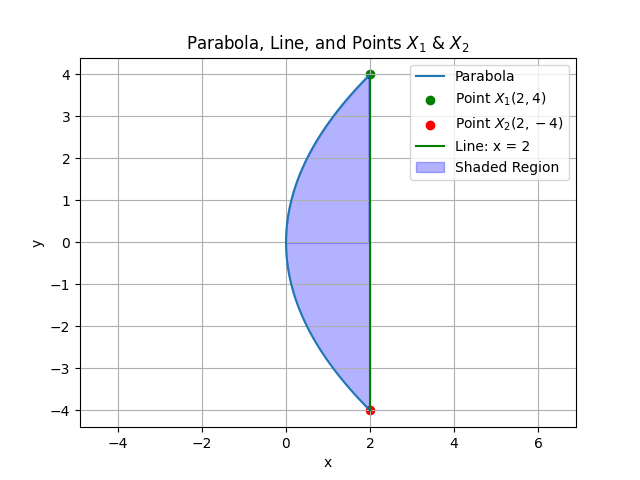
\includegraphics[width = 1\linewidth]{figs/fig.png}
   \caption{The parabola along with the line}
   \label{stemplot}
\end{figure}
\end{document}
